%% And extended abstract addressing:
%% - Problem & motivation
%% - Background & related work
%% - Approach & uniqueness
%% - Results and contributions
%%
%% 2 pages, pdf. Reference lists don't count.
%% Options:
%% - acmart[sigplan]
%% - rntz, rntzgeometry[a5], pdfbook
%%   hm, need custom configuration...

\documentclass[sigplan,screen,dvipsnames]{acmart}
\settopmatter{printacmref=false}
\setcopyright{none}
\renewcommand\footnotetextcopyrightpermission[1]{}
\pagestyle{empty}

\usepackage[scale=0.94]{XCharter}
%\usepackage[scale=0.81]{librebaskerville}%\linespread{.97}
%\usepackage[scale=0.82]{librebaskerville}\linespread{.995}
%\usepackage{eulervm}\makeatletter\edef\zeu@Scale{.975}\makeatother



%% %% ---- Formatting ----
%% \documentclass[twocolumn,10pt]{extarticle}
%% \usepackage[dvipsnames]{xcolor}
%% \usepackage[a4,width=175mm]{rntzgeometry}
%% \setlength\columnsep{20pt}
%% \setlength\parskip{0pt}

%% %% TODO: smaller section titles
%% \usepackage{titlesec}    % (sub)section header styling
%% \titleformat*{\section}{\normalfont\large\bfseries}
%% \titleformat*{\subsection}{\normalfont\normalsize\bfseries}
%% \titlespacing{\section}{0pt}{.667em plus .1em minus .1em}{.3em plus .1em}

%% \usepackage[scale=1.0355]{cochineal}
%% \usepackage[semibold,scaled=.911]{sourcesanspro}
%% %\usepackage{biolinum}
%% \usepackage[scaled=.969]{inconsolata}
%% \usepackage[small]{eulervm}

%% \usepackage[spacing=true]{microtype}
%% \frenchspacing


%% ---- Packages ----
\usepackage{amsfonts,amsmath,latexsym,stmaryrd}
\usepackage{anyfontsize}
\usepackage{lipsum}
\usepackage{mathpartir}
\usepackage{mathtools}          % \dblcolon
\usepackage[nameinlink]{cleveref}
\usepackage{tikz,tikz-cd}
\usepackage{multirow}
\usepackage{booktabs}           % \midrule
\usepackage{nccmath}            % fix spacing issues


%% ---- Commands ----
\newcommand\rulestyle{\sffamily\scshape}
\newcommand\rulename[1]{{\rulestyle#1}}
\newcommand{\catname}[1]{\textbf{#1}}
\newcommand{\Preorder}{\catname{Preorder}}

\newcommand\R{\mathbb{R}}
\newcommand\x\times
\newcommand\todo[1]{{\color{Purple}#1}}
\renewcommand\G\Gamma
\newcommand\D\Delta
\newcommand\mto{\overset{+}{\to}}

\newcommand{\opcolor}{\color{ForestGreen}}
\newcommand{\isocolor}{\color{NavyBlue}}
\newcommand{\pathcolor}{\color{Bittersweet}}

\newcommand{\id}{\textrm{id}}
\newcommand{\op}{\textrm{\opcolor op}}
\newcommand{\iso}{{\texorpdfstring{\ensuremath{\isocolor\Box}}{iso}}}
\renewcommand{\path}{{\texorpdfstring{\ensuremath{\pathcolor\lozenge}}{path}}}

\newcommand{\idof}{\id\,}
\newcommand{\opof}{\op\,}
\newcommand{\isof}{\iso}
\newcommand{\pathof}{\path}

%% TODO: remove these.
\newcommand{\cid}{\id}
\newcommand{\cop}{{\opcolor\op}}
\newcommand{\ciso}{{\isocolor\iso}}
\newcommand{\cpath}{{\pathcolor\path}}

\newcommand\h[3]{#1 : \left[#2\right] #3}
\newcommand\subtype[3]{\left[#1\right] #2 <: #3}

\newcommand\kw[1]{\textrm{#1}}
\newcommand\boxof{\kw{box}~}
\newcommand\elet[1]{\kw{let}~#1~\kw{in}~}
\newcommand\fn\lambda
\newcommand\fnof[1]{\lambda{#1}\binder}
\newcommand\binder{.~}

\newcommand\checksto{~\mathbf{checks}~}
\newcommand\infersto{~\mathbf{infers}~}
\newcommand{\checks}[5]{\h{#1}{#2}{#3} \vdash #4 \checksto #5}
\newcommand{\infers}[5]{\h{#1}{#2}{#3} \vdash #4 \infersto #5}


%% ---- Top matter ----
%%
%% Should include:
%% - Student author's name & email
%% - Institutional affiliation
%% - Research advisor's name
%% - ACM student member number
%% - Category (graduate or undergraduate)
%% - Research title
\title{Type inference for monotonicity}
\author{Michael Arntzenius, a graduate student ...}
\email{daekharel@gmail.com}
\affiliation{University of Birmingham}
\authornote{ACM Student \# TODO}

% arg, should this be Neel or Dan? Neel, probably.
\author{... advised by Neelakantan R. Krishnaswami}
\email{neelakantan.krishnaswami@gmail.com}
\affiliation{University of Cambridge}


\begin{document}

\maketitle


\section{Problem \& motivation}
%% Clearly state the problem being addressed and explain the reasons for seeking
%% a solution to this problem.

Quick: which of these are monotone in $x$?\footnote{Whenever I say ``monotone''
  I mean ``monotonically nondecreasing'': $f$ is monotone iff $x \le y \implies
  f(x) \le f(y)$.}
%
\begin{mathpar}
  x - \log x

  x + 2^x

  {-2}x

  4
\end{mathpar}

Now, how did you \emph{know}?
%
Did you prove from first principles that $x \le y$ implies
%$x + \log x \le y + \log y$?
$x + 2^x \le y + 2^y$?
%
I didn't. I used a shortcut: compositional reasoning. Addition is monotone, and
so is $2^x$; so $x + 2^x$ must be as well.
%
And when I hear ``compositional reasoning'', I think ``type system''.

I aim to give a type system that can statically guarantee a function is monotone.
%
%Moreover, I aim to be able to \emph{infer} whether functions are monotone in their arguments without requiring any annotations other than type annotations.
%
This system is flexible---capable, for example, of typing a function $f : A \x
B \to C$ which is monotone in $A$ but not $B$.
%
It handles several flavors (or \emph{modes}) of function: ordinary (or
\emph{invariant}), monotone, antitone, and bivariant (both mono- and anti-tone).
%
And it requires no changes to terms besides type annotations.

%What use might a type system guaranteeing monotonicity of certain functions be?
%
Monotonicity crops up in a variety of interesting places. In abstract
interpretation, static analyses are phrased as monotone maps on lattices. In
Datafun~\cite{datafun}, monotonicity is needed to ensure that recursive queries
terminate. Monotonicity turns out to be relevant to ensuring eventual
consistency in distributed systems \citep{bloom} and determinism in concurrent
systems \cite{lvars}. In all these cases, the need to ensure monotonicity by one
means or another occurs. Spotting a nail, I offer my favorite hammer: a
type system!


\section{Background \& related work}

%% \todo{
%% Describe the specialized (but pertinent) background necessary to appreciate
%% the work in the context of ICFP areas of interest. Include references to the
%% literature where appropriate, and briefly explain where your work departs
%% from that done by others.
%% }

%% I extend prior work on Datafun~\citep{datafun}, a pure, total functional
%% language inspired by the deductive database language Datalog~\citep{datalog}.
%% %
%% Like Datalog, Datafun allows recursive queries, computed by iteration to a fixed point. To ensure termination, the iterated function must be monotone.
%% %

I extend prior work on Datafun~\cite{datafun}, a pure and total functional
language generalizing the venerable deductive database language Datalog.
Datafun's original type system has \emph{two separate} function types, ordinary
and monotone; it cannot type a function $A \x B \to C$ monotone in $A$ but not
$B$. I aim to lift this restriction. Besides monotonicity, understanding
Datafun's features is not necessary for the present work.

Clancy and Miller's \emph{Monotonicity Types} \citep{monotonicity-types} also
checks various flavors of (non-)monotonicity for certain functions, called
``sfuns'', but they do not permit nesting sfuns inside other sfuns. I impose no
such restriction.

I use bidirectional type checking \cite{bidirectional}, which requires some type
annotations, but is simpler to describe and implement than full Damas-Milner
inference. Bidirectional typing segregates terms into those that can be
\emph{checked} against a type and those whose type may be \emph{inferred}.
Extending the scheme presented here to full type inference is left to future
work.

%% \todo{TODO: Monotonicity Types , variance analysis?, that static analysis someone's pointed out}


\section{Approach \& uniqueness}

I interpret types $A,B$ as preorders (sets equipped with a reflexive, transitive
relation, written $a \le b : A$) and terms and functions as monotone maps. To
handle non-monotone function flavors, I use four unary type operators called
\emph{modes} that alter types' orderings (but not their elements). These are
\id{}, \op{}, \iso{}, and \path{}, defined by:

\[\setlength{\arraycolsep}{.25em}\begin{array}{lll}
  a \le b : \idof A &\iff& a \le b : A\\
  a \le b : \opof A &\iff& a \ge b : A\\
  a \le b : \isof A &\iff& a \le b \wedge a \ge b : A\\
  a \le b : \pathof A &\impliedby& a \le b \vee b \le a : A
\end{array}\]

Each mode captures a function flavor: \id{} for monotone, \op{} for antitone,
\iso{} for invariant, and \path{} for bivariant. For example, $f : A \to B$ is
antitone iff $f : \opof{A} \to B$ is monotone. Moreover, we can mix-and-match:
$A \x \isof{B} \to C$ denotes functions monotone in $A$, but invariant in $B$.

$\iso$ and $\path$ are necessity and possibility modalities in the sense of
\citet{jrml}. Invoking Curry-Howard, we may endow their rules for $\iso$ and
$\path$ with proof terms. But I want to \emph{avoid} explicit term syntax for
modal types.
%
For example, given $(-) : \R \x \isof{\R} \to \R$ and $\log : \isof{\R} \to \R$,
I'd like to write $(\fnof{x} x - \log x) : \isof\R \to \R$. With their rules, it
would look more like $(\fnof{x} \elet{\boxof u = x} u - \boxof(\log x))$.
%
I avoid this bureaucracy with two simple tricks:
\begin{enumerate}
\item Infer variable usage modes bottom-up.
\item Use \emph{modal subtyping} to silently convert to and from modal types.
\end{enumerate}

In the remainder of this section, I sketch how these tricks apply to a tiny
fragment (\cref{fig:rules,fig:mode-ops}) of the type system I have constructed.


\subsection{Inferring variable usage modes}

\begin{figure}
  \begin{mathpar}
    %\setlength{\arraycolsep}{.3em}
    %% \begin{array}{rc@{\hskip .67em}c@{\hskip .67em}l}
    %%   \text{modes} & T,U &\dblcolon=& \id ~|~ \op ~|~ \iso ~|~ \path\\
    %%   \text{types} & A,B &\dblcolon=& A \x B ~|~ TA ~|~ ...\\
    %%   \text{expressions} & e &\dblcolon=& (e,e) ~|~ \elet{x = e} e ~|~ ...
    %% \end{array}
    %%
    \infer[\rulestyle pair]{
      \checks{x}{T}{A}{e_1}{B_1} \\
      \checks{x}{U}{A}{e_2}{B_2}
    }{
      \checks{x}{T\wedge U}{A}{(e_1,e_2)}{B_1 \x B_2}
    }

    \infer[\rulestyle let]{
      \infers{x}{T}{A}{e_1}{B} \\
      \checks{y}{U}{B}{e_2}{C}
    }{
      \checks{x}{UT}{A}{\elet{y = e_1} e_2}{C}
    }

    \infer[\rulestyle subsumption]{
      \infers{x}{T}{A}{e}{B} \\ \subtype{U}{B}{C}
    }{\checks{x}{UT}{A}{e}{C}}
\\
    \infer[\rulestyle $\iso$-injection]{
      \subtype{T}{A}{B}
    }{
      \subtype{\iso T}{A}{\isof B}
    }

    \infer[\rulestyle $\iso$-extraction]{\subtype T A B}{
      \subtype{\path}{\isof A}{B}
    }
  \end{mathpar}
  \caption{Example typing and subtyping rules}
  \label{fig:rules}
\end{figure}

\begin{figure}
  \begin{mathpar}
    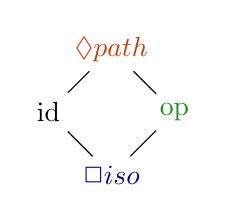
\begin{tikzpicture}[scale=0.8,baseline=(current bounding box.center)]
      \node (top)  at ( 0, 1) {$\cpath$};
      \node (bot)  at ( 0,-1) {$\ciso$};
      \node (-1)   at (-1, 0) {$\cid$};
      \node (1)    at ( 1, 0) {$\cop$};
      \draw (top) -- (-1) -- (bot) -- (1) -- (top);
    \end{tikzpicture}
    %%
    %% \begin{array}{r|cccc}
    %%   T \wedge U
    %%   & \cid & \cpath & \cop & \ciso\\\hline
    %%   \cid & \cid & \cid & \ciso & \ciso\\
    %%   \cpath & \cid & \cpath & \cop & \ciso\\
    %%   \cop & \ciso & \cop & \cop & \ciso\\
    %%   \ciso & \ciso & \ciso & \ciso & \ciso
    %% \end{array}

    \begin{array}{cr|cccc}
      \multicolumn{2}{c|}{\multirow{2}{*}{$UT$}}
      & \multicolumn{4}{c}{T}\\
      && \cid & \cop & \ciso & \cpath\\\hline
      \multirow{4}{*}{$U$}
      & \cid & \cid & \cop & \ciso & \cpath\\
      & \cop & \cop & \cid & \ciso & \cpath\\
      & \ciso & \ciso & \ciso & \ciso & \cpath\\
      & \cpath & \cpath & \cpath & \ciso & \cpath
    \end{array}
  \end{mathpar}

  \caption{Mode lattice and composition}
  \label{fig:mode-ops}
\end{figure}


I use two typing judgments: $\G \vdash e \infersto B$, where $B$ is an
\emph{output} of the rule, and $\G \vdash e \checksto B$, where it is an
\emph{input}. The full system handles many variables, but to simplify my
examples, I restrict to single-variable contexts, $\G \dblcolon= \h x T A$. A
variable $x$ has both a type $A$ and a mode $T$ saying \emph{how} it is used.
$A$ is (as usual in bidirectional typing) an input, but $T$ is an
\emph{output}---we infer how variables are used!

\rulename{pair} (\cref{fig:rules}) shows how this \emph{mode inference} works
when a variable is used multiple times. If $x$ is used in $e_1, e_2$ at modes
$T,U$ respectively, then $(e_1,e_2)$ uses $x$ at their \emph{meet}, $T \wedge
U$, in the lattice shown in \cref{fig:mode-ops}. The ordering of the mode
lattice arises naturally as follows. For preorders $A,B$, let $A \le B$ iff $A$
is a subpreorder of $B$ (iff $A \subseteq B$ and $x \le y : A \implies x \le y :
B$). Then $T \le U$ iff $\forall A.~ TA \le UA$. So $T \wedge U$ is the most
general mode which supports both uses at mode $T$ and at $U$.

\rulename{let} (\cref{fig:rules}) shows how mode inference works under
\emph{composition} of computations: if $x$ is used at mode $T$ to compute $e_1$,
which is bound to $y$ and used at mode $U$ to compute $e_2$, the overall
expression uses $x$ at the composition of modes $UT$ (\cref{fig:mode-ops}) such
that $(UT)A \equiv U(TA)$ (that is, they denote the same preorder).


\subsection{Modal subtyping}

To construct or use terms of modal type $TA$ implicitly, I use a subtyping
judgment, $\subtype{T}{A}{B}$. Given input types $A,B$ this outputs the
\emph{greatest} mode $T$ such that $TA \le B$ (if one exists).
\rulename{subsumption} lets a term $e : B$ be used at type $C$ by
\emph{composing} it with the subtyping $\subtype{U}{B}{C}$. This composes $U$
onto the context: subtyping changes variables' usage modes!

Compared to a typical subtyping judgment $A <: B$, this extra degree of freedom
lets us silently coerce into and out of $\isof A$ using
\rulename{$\iso$-injection} and \rulename{$\iso$-extraction} (\cref{fig:rules}).
\rulename{$\iso$-injection} internalizes $\iso$'s covariance, while
\rulename{$\iso$-extraction} uses the properties $\forall T.~ \iso \le T$ and
$\path\iso = \iso$.


\subsection{Novelty}

I have not surveyed the entire literature, but I know of no other modal type
system where subtyping alters the typing context, the ``trick'' I use to
silently coerce to and from modal types. Although not discussed here, I also
handle pattern-matching by distributing modes over products and sums. These
tricks let us generalize Datafun by handling function types like $A \x \iso B
\to C$, which are monotone in $A$ but not $B$, \emph{without} additional term
syntax. We also generalize \citet{monotonicity-types} by handling
nested $\fn$-abstractions.

%% \todo{Describe your approach in addressing the problem and clear\-ly state how
%%   your approach is novel.}

%% - interpret everything in Preorder
%%
%% - infer how variables are used, entirely bottom-up (novel!)
%%
%% - use modal subtyping to handle mismatches between inferred & expected types, and to handle function application (novel!)
%%
%% - use distribution of modes to handle pattern-matching (novel?)

%% novel: modes for monotonicity! (not special kinds of functions, as in Datafun & Monotonicity Types)
%%
%% novel: higher-order! unlike Monotonicity Types!
%%
%% no intro/elim annotations! unlike Pfenning-Davies, certainly, or basically any modal approach?

%% but how does it differ from variance typing? well, variance typing in e.g.
%% Agda at least is mostly not exposed to the user. in OCaml it is but OCaml
%% doesn't have a full type-level programming language.


\section{Results and contributions}
%% \todo{Clearly show how the results of your work contribute to programming
%%   language design and implementation in particular and to computer science in
%%   general; explain the significance of those results.}

I construct a simply-typed modal $\fn$-calculus with a denotational semantics in
the category of preorders and monotone maps. I aim to prove (but haven't yet)
that typing is preserved under substitution and subtyping. From these, the
derivability of the rules in \citet{jrml} follows. I also hope to prove that
every Datafun program typechecks in my system with no changes except local
rewriting of types. This would achieve my primary goal: to make Datafun more
flexible.

More generally, my system could provide a jumping-off point for systems which
need to ensure monotonicity for other reasons, such as for static analysis or
eventual consistency.

Finally and most speculatively, the combination of inferring variable modes and
modal subtyping might prove useful for eliminating bureaucratic term syntax in
other modal languages. Modal subtyping in particular may have wide application:
modal type systems manipulate the context, so allowing subtyping to manipulate
it as well is a natural fit. Modal types occur in languages for reactive
programming \cite{Krishnaswami13:simple-frp}, distributed programming
\cite{ml5}, and resource-constrained programming
\cite{context-constrained,DBLP:conf/esop/GhicaS14}; could these techniques make
such languages more flexible and less verbose? The only way to find out is to
try.

%% Results: a type system with a formal semantics in Preorder. WTB: formal proof of substitution and subtyping lemmas. from these, derivability of Pfenning-Davies rules follows. want to show: everything typable in Datafun typechecks, rewriting only types.

% Makes Datafun more flexible.
% - functions f : A * B -> C
% - handles antitonicity for e.g. parity-stratified negation
% - no need to annotate case-expressions

% Suggests a novel approach to modal type systems that could, in some
% circumstances, result in fewer annotations and more ``natural'' code.


%% Bibliography
\bibliographystyle{abbrvnat}
\bibliography{datafun}

\end{document}
